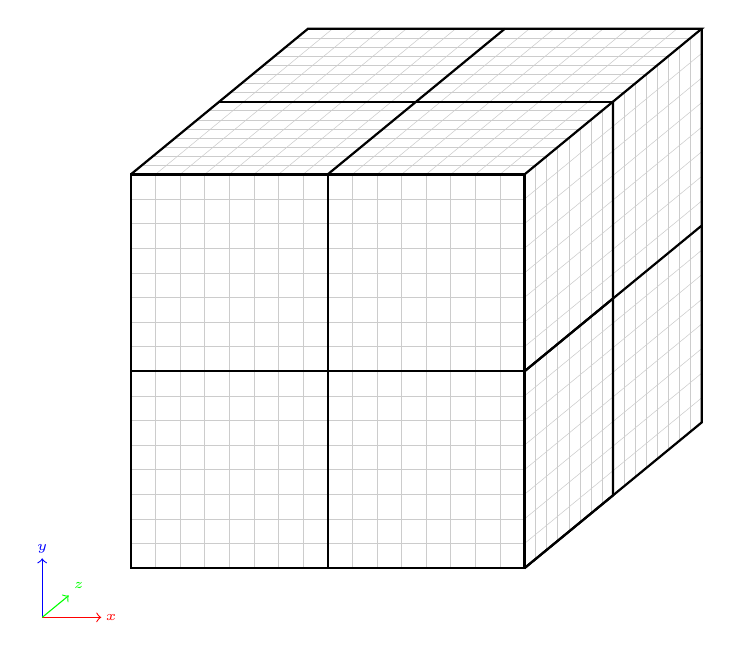
\begin{tikzpicture}[z={(-0.45cm,-0.37cm)}, scale=2.5]

\tikzstyle{inner} = [gray!40!white,very thin]
%front face vertical
\foreach \x in {1,2,3,4,5,6,7,9,10,11,12,13,14,15}
  \draw[inner] (\x/8,0) -- (\x/8,2);
%front face horizontal
\foreach \x in {1,2,3,4,5,6,7,9,10,11,12,13,14,15}
  \draw[inner] (0,\x/8) -- (2,\x/8);

%rigt face vertical
\foreach \x in {1,2,3,4,5,6,7,9,10,11,12,13,14,15}
  \draw[inner] (2,0,-\x/8) -- (2,2,-\x/8);
%rigth face horizontal
\foreach \x in {1,2,3,4,5,6,7,9,10,11,12,13,14,15}
  \draw[inner] (2,\x/8,0) -- (2,\x/8,-2);

%top face front to back
\foreach \x in {1,2,3,4,5,6,7,9,10,11,12,13,14,15}
  \draw[inner] (\x/8,2,0) -- (\x/8,2,-2);
%top face left to rigth
\foreach \x in {1,2,3,4,5,6,7,9,10,11,12,13,14,15}
  \draw[inner] (0,2,-\x/8) -- (2,2,-\x/8);


\draw[thick] (0,0) rectangle (1,1);
\draw[thick] (1,0) rectangle (2,1);
\draw[thick] (0,1) rectangle (1,2);
\draw[thick] (1,1) rectangle (2,2);

\draw[thick] (2,1) -- (2,1,-1) -- (2,2,-1);
\draw[thick] (2,1) -- (2,1,-2) -- (2,2,-2);
\draw[thick] (2,0) -- (2,0,-1) -- (2,1,-1);
\draw[thick] (2,0) -- (2,0,-2) -- (2,1,-2);

\draw[thick] (1,2) -- (1,2,-2);
\draw[thick] (0,2,-1) -- (2,2,-1);

\draw[thick] (0,2) -- (0,2,-2) -- (2,2,-2) -- (2,2);

\draw[red,->] (-0.45,-0.25) -> (-0.15,-0.25) ;
\draw[red] (-0.1, -0.25) node[font=\tiny] {$x$};

\draw[blue,->] (-0.45,-0.25) -> (-0.45, 0.05);
\draw[blue] (-0.45, 0.1) node[font=\tiny] {$y$};


\draw[green,->] (-0.45,-0.25) -> (-0.45, -0.25, -0.3);
\draw[green] (-0.40, -0.20, -0.3) node[font=\tiny] {$z$};

\end{tikzpicture}